\documentclass{article}
\usepackage{tikz}
\usetikzlibrary{graphs,intersections,math,animations}

\begin{document}

\begin{figure}
  \begin{center}
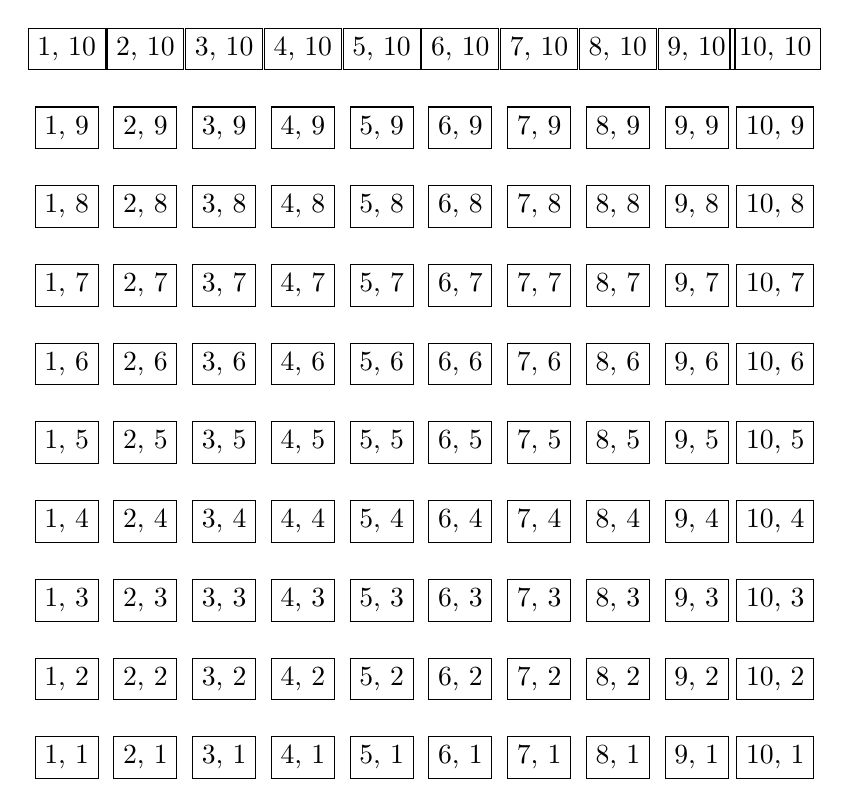
\begin{tikzpicture}
  \node foreach \x in {1,...,10} foreach \y in {1,...,10}
       [draw] at (\x, \y) {\x, \y};
\end{tikzpicture}
  \end{center}
  \caption{}
  \label{fig:}
\end{figure}

\begin{figure}
  \begin{center}
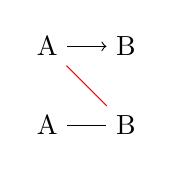
\begin{tikzpicture}
\begin{scope}[name prefix = top-]
    \node (A) at (0,1) {A};
    \node (B) at (1,1) {B};
    \draw[->] (A) -- (B);
\end{scope}
\begin{scope}[name prefix = bottom-]
    \node (A) at (0,0) {A};
    \node (B) at (1,0) {B};
    \draw (A) -- (B);
  \end{scope}
  \draw [red] (top-A) -- (bottom-B);

\end{tikzpicture}
  \end{center}
  \caption{}
  \label{fig:}
\end{figure}

\begin{figure}
  \begin{center}
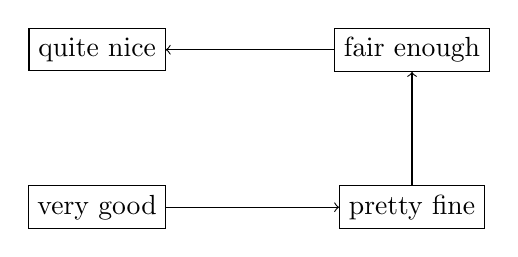
\begin{tikzpicture}[every node/.style={draw}]
  \path[shape=rectangle]
(0,0) node(a1){very good}
(4,0) node(a2){pretty fine}
(4,2) node(a3){fair enough}
(0,2) node(a4){quite nice};
\draw[->] (a1) -- (a2);
\draw[->] (a2) -- (a3);
\draw[->] (a3) -- (a4);
\end{tikzpicture}
  \end{center}
  \caption{}
  \label{fig:}
\end{figure}


\end{document}
